\chapter{Ausblick}
Es wurden bereits die Vorteile und Nachteile des VAE basierten Ansatzes der Data Augmentation vorgeführt. Im anschließenden Kapitel wird ein Ausblick über Weiterentwicklung der in dieser Arbeit vorgestellten Konzepte gegeben. \\

\section{Few-Shot Learning}
In der vorliegenden Arbeit wurde beobachtet, dass die verwendeten Augmentierungs Techniken, besonders im Few-Shot Szenario zu konsistenten Verbesserungen führten. Man beachte, dass diese Verbesserungen ausschließlich über Data Augmentation erzielt und keine Few-Shot Learning spezifischen Ansätze verwendet wurden. Eine vielversprechende Idee ist daher, die VAE basierte Data Augmentation mit \textit{State-of-the-Art} Few-Shot Learning Ansätzen, wie "Transfer-Learning" und "Meta-Learning", zu kombinieren.


%\section{Multi-Label Klassifikation}
%Die Multi-Label Klassifikationsaufgabe geht über den Fokus dieser Arbeit hinaus. Dennoch stellt sich die Frage, inwiefern die Klassifikation verbessert werden kann, wenn die Daten eines Distentangled-VAE hinzugenommen werden. Außerdem repräsentieren die Dimensionen des Latent-Space nicht alle gelernten Merkmale. \cite{Klys2018} liefern einen Ansatz, um besser Subräume im Latent-Space zu finden, die Attributen im Datensatz entsprechen.
\section{Weitere VAE Modelle}
\subsection{Denoising und Conditional VAE}
Für die Anwendung von VAE Modellen auf den numerischen Daten des PROBEN1 Datensatzes, wurden von \cite{Moreno-Barea2020} zwei Weiterentwicklungen vorgestellt: Der Denoising-VAE (DVAE) und der Conditional-VAE (CVAE). Der DVAE hat dieselbe Funktionsweise wie schon der in Abschnitt \ref{sec:dae} angeführte Denoising Autoencoder. Das Eingabebeispiel $x$ wird durch eine modifizierte Variante $\tilde{x}$ ersetzt. Der CVAE gibt dem VAE zusätzlich zum gesampelten $z$ die Klassen Information $y$ mit. Die Ausgabeverteilung des Encoders und Decoders hängt somit jeweils auch von der Klasse des gesampelten Latent-Vektors ab. Die Fehlerfunktion von DVAE und CAE haben folgende Form:
\begin{align}
  \cL_{\textit{DVAE}} &= \bE \left[\log P_\theta(x \vert z) - \cD_{KL}\left[Q_\phi(z \vert \tilde{x}) \| \cN(0, 1)\right] \right] \\[6pt]
  \cL_{\textit{CVAE}} &= \bE \left[\log P_\theta(x \vert z, y) - \cD_{KL}\left[Q_\phi(z \vert x, y) \| \cN(0, 1)\right] \right]
\end{align}


\subsection{VAE-GAN}
\cite{Larsen2016} schlagen in ihrer Arbeit eine Kombination des VAE Modells mit einem Generative-Adversarial-Network (GAN) vor. GANs erzeugen wesentlich schärfere Bilder, haben aber keinen Encoder. Dies hat zur Folge, dass sie weniger Kontrolle über die Rekonstruktionen bieten, da keine Manipulationen im Latent-Space möglich sind. Das vorgeschlagene VAE-GAN Modell kombiniert den Encoder des VAEs mit der Generator-Discriminator Architektur des GANs, indem der Decoder durch den Generator und Discriminator ersetzt wird (siehe Abb. \ref{fig:vae_gan}). VAE-GANs haben die gleichen Latent-Space Eigenschaften wie VAEs, erzeugen aber wesentlich schärfere Bilder, wie in Abb. \ref{fig:vae_gan_reconstruction} zu sehen ist. Damit führen die Autoren die Vorteile dieser beiden generativen Ansätze in einem Modell zusammen.

%Ein GAN besteht aus zwei Netzwerken: Einem Generator und ein Discriminator (siehe auch \cite{goodfellow2014generative}. Der Generator bildet Elemente $z$ aus dem Latent-Space auf ein $\hat{x}$ in den Raum der Daten ab. Der Discriminator bewertet, ob das erzeugte Beispiel ein "echtes" Trainingsbeispiel oder ein generiertes Beispiel ist. Beide Netzwerke optimieren sich gegenseitig über folgende Fehlerfunktion:
%\begin{equation}
%  \cL_{GAN} = \log Dis(x) + \log(1 - Dis(Gen(z)),
%\end{equation}
%mit $x \sim D$ Datensatz und $z \sim P(z)$.\\

\begin{figure}[hbt]
\centering
  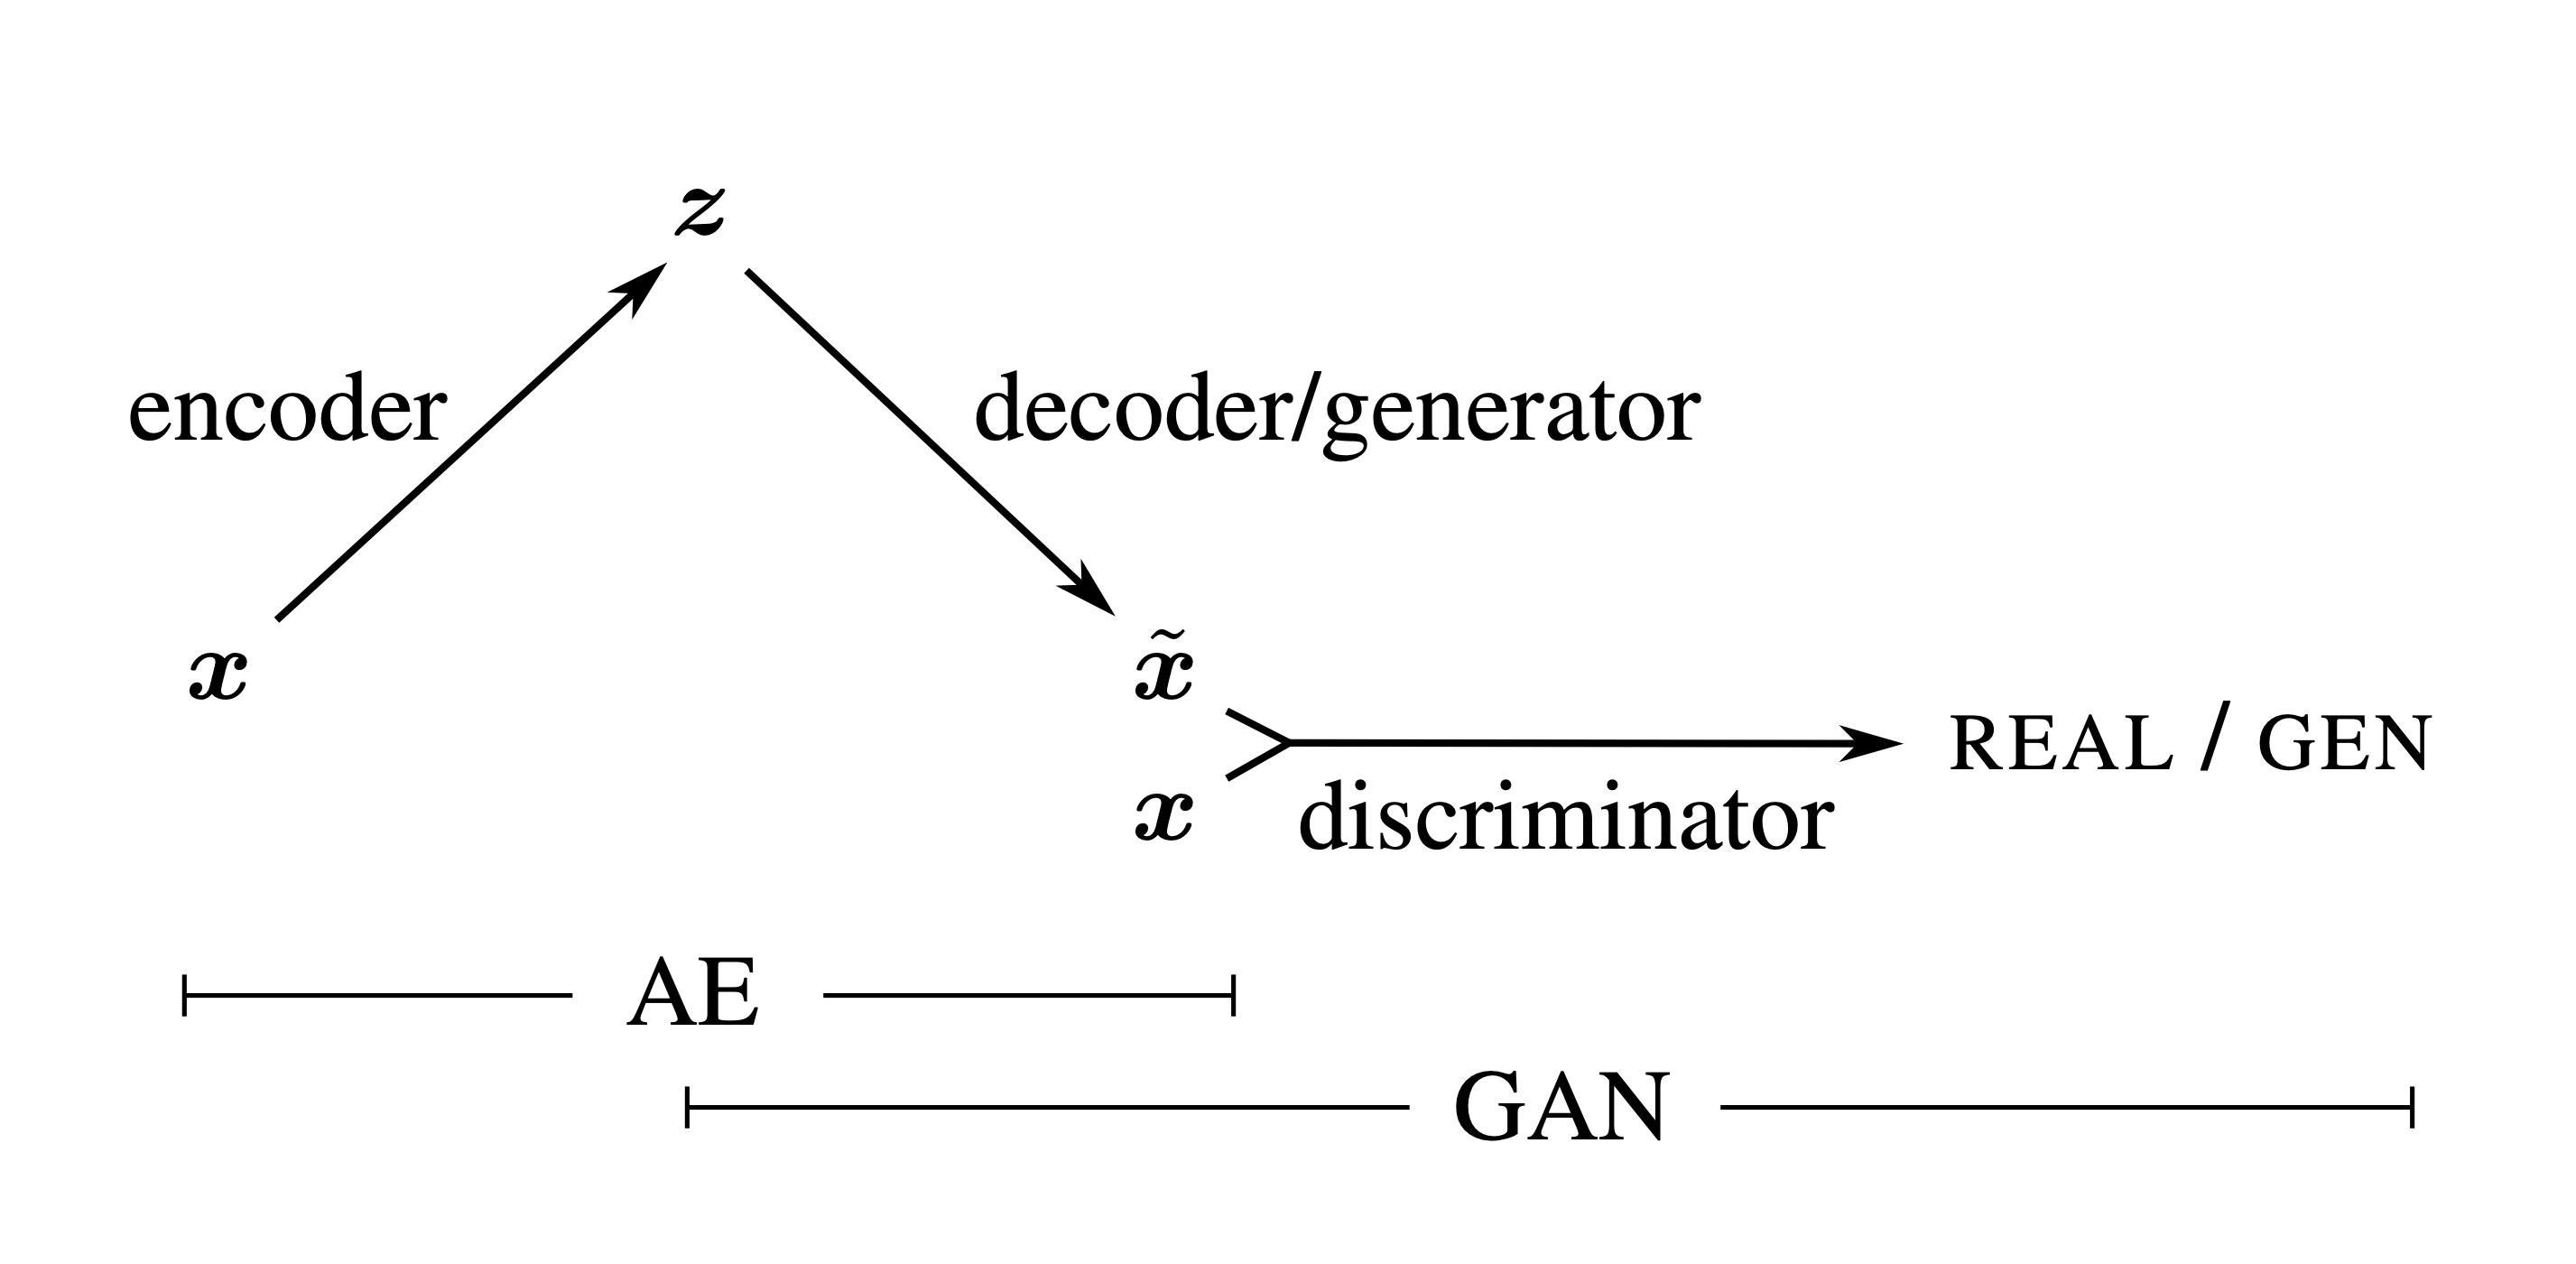
\includegraphics[width=.7\textwidth]{gfx/outlook/vae_gan}
  \caption{Das VAE-GAN Modell. Der Decoder des VAEs wird durch den Generator und den Discriminator ersetzt. Abbildung entnommen aus \cite{Larsen2016}}
  \label{fig:vae_gan}
\end{figure}

\begin{figure}[hbt]
\centering
  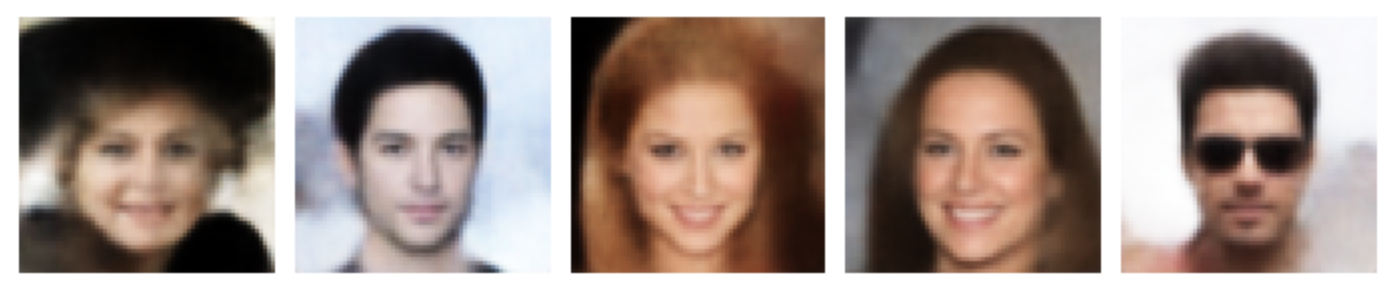
\includegraphics[width=.7\textwidth]{gfx/outlook/ours}
  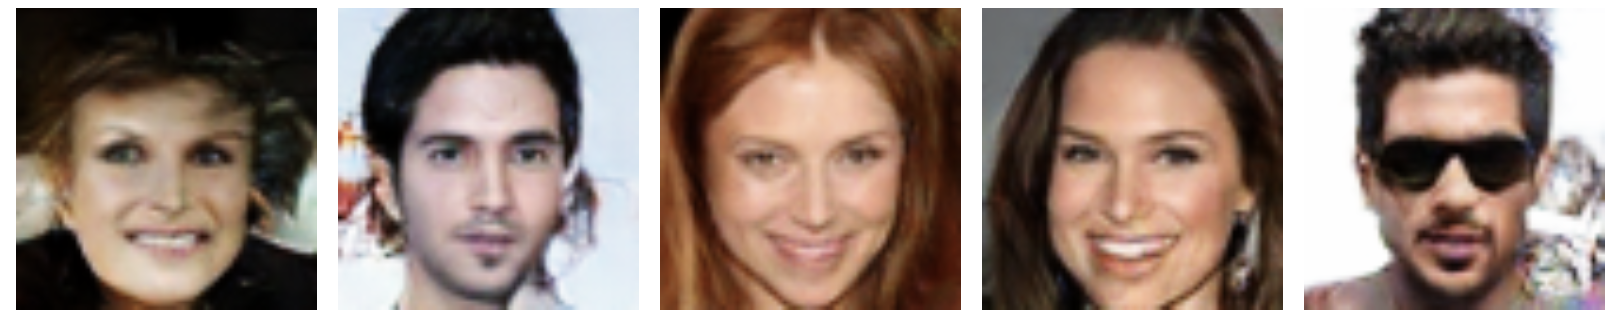
\includegraphics[width=.7\textwidth]{gfx/outlook/vae_gan_reconstruction}
  \caption{Die Rekonstruktionen unseres VAE Modells (oben). Die Rekonstruktionen des VAE-GAN Modells (unten) (VAE-GAN Bilder entnommen aus \cite{Larsen2016})}
  \label{fig:vae_gan_reconstruction}
\end{figure}
